\documentclass[10pt,twocolumn]{article}

% -------------------------------------------------------------
% Packages
% -------------------------------------------------------------
\usepackage[margin=0.70in,top=0.75in,bottom=0.75in]{geometry}
\usepackage{lmodern}
\usepackage{amsmath,amssymb,amsfonts}
\usepackage{graphicx}
\usepackage{booktabs}
\usepackage{tabularx}
\usepackage{array}
\usepackage{xcolor}
\usepackage{url}
\usepackage{cite}
\usepackage[hidelinks,colorlinks=true,linkcolor=blue!70!black,citecolor=blue!70!black,urlcolor=blue!70!black]{hyperref}

% Define color palette
\definecolor{primary}{RGB}{13, 27, 42}
\definecolor{accent}{RGB}{0, 119, 182}
\definecolor{success}{RGB}{42, 157, 143}
\definecolor{danger}{RGB}{231, 111, 81}

% Formatting tweaks
\setlength{\columnsep}{0.25in}
\setlength{\parskip}{0pt}
\setlength{\parindent}{11pt}

% Section styling
\makeatletter
\renewcommand\section{\@startsection {section}{1}{\z@}%
  {-2.0ex \@plus -0.5ex \@minus -.2ex}%
  {1.0ex \@plus .2ex}%
  {\normalfont\normalsize\bfseries\scshape\color{primary}}}
\renewcommand\subsection{\@startsection{subsection}{2}{\z@}%
  {-1.5ex\@plus -0.4ex \@minus -.2ex}%
  {0.6ex \@plus .2ex}%
  {\normalfont\normalsize\bfseries\itshape\color{accent}}}
\renewcommand\subsubsection{\@startsection{subsubsection}{3}{\z@}%
  {-1.0ex\@plus -0.3ex \@minus -.2ex}%
  {0.4ex \@plus .2ex}%
  {\normalfont\small\bfseries}}
\makeatother

% -------------------------------------------------------------
% Document Metadata
% -------------------------------------------------------------
\title{\vspace{-0.3in}\textbf{\Large A Privacy-Preserving Cloud Data Sharing Architecture for Multi-Hospital Electronic Health Records: Integrating Searchable Encryption, Multi-Authority ABAC, Proxy Re-Encryption, and Dynamic Behavioral Trust}}

\author{
  \textbf{Divyanshu} (\texttt{23BEC017}) \quad $\vert$ \quad
  \textbf{Adnan Khan} (\texttt{23BEC028}) \quad $\vert$ \quad
  \textbf{Harshit Tripathi} (\texttt{23BCS054})\\[3pt]
  \small Indian Institute of Information Technology Dharwad\\
  \small Course: Cloud SRE and Security \quad $\vert$ \quad Supervisor: Prof. Malay Kumar\\[1pt]
  \small Theoretical Foundation: Pan Jun Sun, \textit{IEEE Access}, vol. 7, 2019 \cite{sun2019privacy}
  \vspace{-0.15in}
}

\date{}

% -------------------------------------------------------------
% Begin Document
% -------------------------------------------------------------
\begin{document}

\maketitle

\begin{abstract}
\textbf{\textit{Abstract}---Cloud-based healthcare data sharing enhances diagnostic velocity and multi-institutional collaboration but introduces severe security and privacy vulnerabilities when electronic health records (EHRs) are outsourced to semi-trusted public cloud service providers (CSPs). Guided by the cloud privacy taxonomy formalized by Pan Jun Sun (IEEE Access 2019), this paper presents \textit{MediCloud}, an end-to-end privacy-preserving cloud storage and sharing architecture designed for federated hospital ecosystems. MediCloud realizes an interlocking defense-in-depth framework incorporating five core cryptographic and site reliability engineering (SRE) primitives: (1) AES-256-GCM authenticated encryption with Additional Authenticated Data (AAD) record binding; (2) Searchable Symmetric Encryption (SSE) via blind HMAC-SHA256 inverted trapdoor indexes; (3) Decentralized Multi-Authority Attribute-Based Access Control (MA-ABAC); (4) BBS98 Proxy Re-Encryption (PRE) over RFC 3526 1024-bit MODP safe prime fields for cloud-delegated, $O(1)$ client-bandwidth staff revocation; (5) Dynamic Behavioral Trust and Reputation telemetry enforcing continuous exponential decay ($e^{-\lambda \Delta t}$) and automated quarantine gating below a $0.40$ threshold; (6) Cryptographic traitor tracing for rogue key leak accountability; and (7) Tamper-evident SHA-256 audit logging. The prototype was evaluated across 16 functional security test cases, achieving a 100\% verification rate (16/16 passed). Empirical microbenchmarks confirm sub-millisecond execution times ($\approx 0.48$~ms upload pipeline, $\approx 0.056$~ms decryption, and $\approx 0.0026$~ms search), demonstrating that production-grade cloud confidentiality and fine-grained access governance can be achieved with negligible operational overhead.}
\end{abstract}

\vspace{4pt}
\noindent\textbf{\textit{Index Terms}---Cloud Security, Privacy-Preserving EHR, Attribute-Based Access Control, Searchable Symmetric Encryption, Proxy Re-Encryption, Behavioral Trust, Site Reliability Engineering.}

% -------------------------------------------------------------
% Section I: Introduction
% -------------------------------------------------------------
\section{Introduction}
Modern healthcare infrastructure increasingly relies on multi-hospital consortia to exchange patient medical histories, diagnostic imaging, and laboratory results. Cloud service providers (CSPs) offer elastic storage and computational scale, making them ideal backbones for cross-institutional Electronic Health Record (EHR) management. However, public cloud infrastructure is inherently \textit{semi-trusted} or \textit{honest-but-curious}: cloud providers faithfully follow communication protocols and execute stored procedures, but possess strong technical ability and commercial incentives to inspect sensitive plaintext medical records. 

Furthermore, multi-tenant cloud virtualization creates persistent attack surfaces for co-tenant data leakage, hypervisor vulnerabilities, and administrative insider threats. Legal and regulatory frameworks---such as HIPAA in the United States, GDPR in the European Union, and the Digital Personal Data Protection (DPDP) Act in India---mandate stringent data isolation, cryptographic confidentiality at rest, granular role separation, and tamper-evident auditing.

In his comprehensive IEEE Access survey, Pan Jun Sun \cite{sun2019privacy} established that no single security primitive suffices to resolve cloud privacy challenges. Complete cloud protection requires an interlocking defense-in-depth architecture combining:
\begin{enumerate}
    \item \textbf{Access Control:} Expressive policy enforcement separating administrative roles from clinical access;
    \item \textbf{Cryptographic Enforcement:} Attribute-Based Encryption (ABE) and Proxy Re-Encryption (PRE) ensuring privacy even against privileged cloud operators;
    \item \textbf{Searchable Encryption (SSE):} Efficient searching over ciphertexts without client-side decryption;
    \item \textbf{Behavioral Trust Systems:} Continuous reputation monitoring to counter credential theft and lateral insider reconnaissance.
\end{enumerate}

To operationalize Sun's theoretical framework, we designed and implemented \textbf{MediCloud}, a production-ready, verified cloud security prototype for multi-hospital EHR exchange. MediCloud translates theoretical cryptographic schemes into practical, high-throughput software components capable of operating on standard cloud computing infrastructure.

\begin{figure*}[!t]
  \centering
  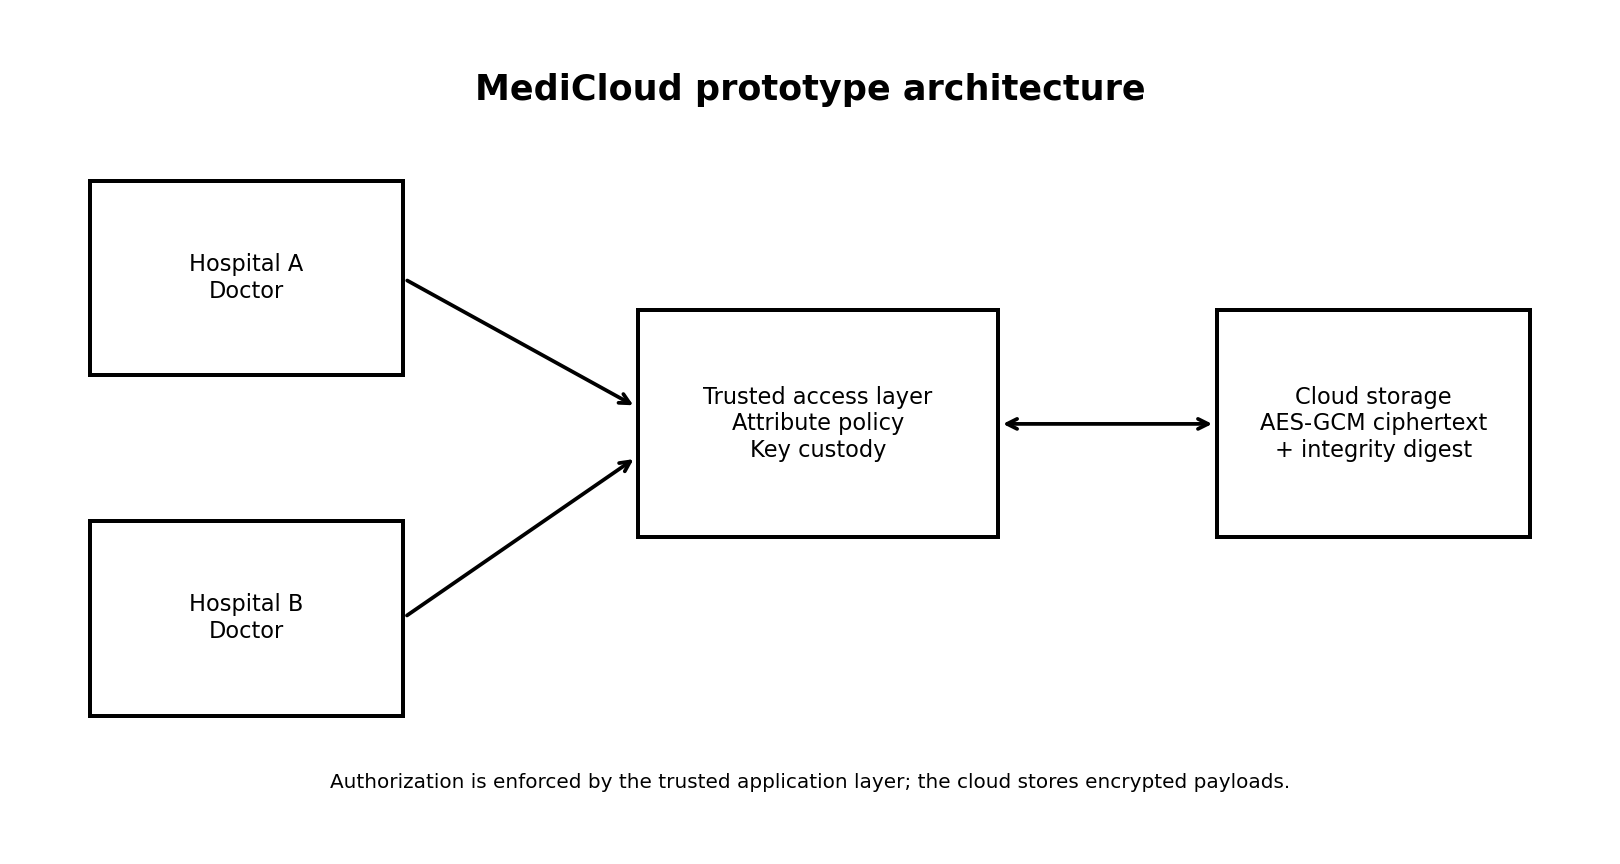
\includegraphics[width=0.92\textwidth]{figures/architecture.png}
  \caption{MediCloud system topology, cryptographic trust boundaries, and multi-hospital interaction flow between Hospital-A, Hospital-B, Diagnostic Laboratories, the Central Medical Council, and the semi-trusted Cloud Repository.}
  \label{fig:arch}
\end{figure*}

% -------------------------------------------------------------
% Section II: Literature Review & Theoretical Foundation
% -------------------------------------------------------------
\section{Literature Review \& Background}
Sun's survey \cite{sun2019privacy} categorizes cloud privacy into four foundational dimensions: access control models, attribute-based cryptographic primitives, searchable encryption schemes, and trust/reputation mechanisms.

\subsection{Access Control Models: DAC, MAC, RBAC, and ABAC}
Early cloud architectures relied on Discretionary (DAC) and Mandatory Access Control (MAC), which fail in multi-tenant environments due to administrative rigidity and inability to scale across administrative boundaries. Role-Based Access Control (RBAC) simplifies role assignment but suffers from ``role explosion'' in federated healthcare where a user's permissions depend on dynamic contextual variables (e.g., hospital affiliation, emergency shift, department). Attribute-Based Access Control (ABAC) resolves this by evaluating Boolean access rules over user, resource, and environmental attributes. However, software-level ABAC implemented by cloud databases leaves records vulnerable to database administrators and compromised storage engines.

\subsection{Ciphertext-Policy ABE vs. Key-Policy ABE}
To bind access policies directly to data, Sahai and Waters pioneered Attribute-Based Encryption (ABE). Goyal et al. \cite{goyal2006attribute} classified ABE into:
\begin{itemize}
    \item \textbf{Key-Policy ABE (KP-ABE):} Ciphertexts are labeled with attribute sets, while user decryption keys encode access trees. KP-ABE suits content distribution but strips data owners of granular control over who reads their files.
    \item \textbf{Ciphertext-Policy ABE (CP-ABE):} Data owners embed access formulas directly into the ciphertext packaging, while user keys represent certified attribute sets. CP-ABE preserves owner sovereignty over healthcare records.
\end{itemize}
Despite its theoretical elegance, standard CP-ABE incurs high pairing latency and suffers from the \textit{centralized authority vulnerability} and \textit{revocation overhead}: revoking a single doctor requires re-encrypting entire cloud archives.

\subsection{BBS98 Proxy Re-Encryption (PRE)}
To solve the revocation bottleneck without requiring data owners to download and re-encrypt cloud archives, Blaze, Bleumer, and Strauss \cite{blaze1998divertible} introduced atomic Proxy Re-Encryption (PRE). An authority computes a re-encryption key $rk_{A \to B}$ from private key $sk_A$ and public key $pk_B$. A semi-trusted proxy applies $rk_{A \to B}$ to translate ciphertexts encrypted under $pk_A$ into ciphertexts decryptable by $sk_B$, without learning the underlying plaintext.

\subsection{Searchable Symmetric Encryption (SSE)}
Outsourcing encrypted files typically precludes server-side search. Curtmola et al. \cite{curtmola2006searchable} formalized Searchable Symmetric Encryption (SSE) utilizing inverted indexes and cryptographic trapdoors. Clients submit blind tokens, enabling the cloud to return matching record IDs with zero plaintext knowledge.

% -------------------------------------------------------------
% Section III: MediCloud Architectural Design
% -------------------------------------------------------------
\section{MediCloud Architectural Design}
Fig.~\ref{fig:arch} depicts the architectural topology and trust boundaries of MediCloud. The system incorporates four primary participant roles:
\begin{enumerate}
    \item \textbf{Data Owners / Clinicians:} Healthcare providers who encrypt, upload, search, and retrieve EHR records.
    \item \textbf{Decentralized Attribute Authorities:} Independent bodies responsible for verifying qualifications and issuing cryptographically signed attribute credentials.
    \item \textbf{Semi-Trusted Cloud Provider:} Commercial hosting infrastructure managing ciphertext objects, blind trapdoor indexes, and re-encryption tasks.
    \item \textbf{Audit \& Trust Authority:} Telemetry engine monitoring request integrity and maintaining append-only access ledgers.
\end{enumerate}

\subsection{Client-Side Authenticated Encryption with AAD Binding}
Every clinical record payload $M$ is encrypted client-side using AES-256 in Galois/Counter Mode (GCM). For each record, a fresh 96-bit cryptographic nonce $N$ is drawn from operating system entropy:
\begin{equation}
    (C, \tau) = \text{AES-GCM-Encrypt}_{DEK}(N, M, AAD)
\end{equation}
where $DEK$ is a 256-bit Data Encryption Key, and $\tau$ is the 128-bit authentication tag. Crucially, the unique record identifier (e.g., \texttt{"ehr001"}) is supplied as Additional Authenticated Data ($AAD$). This mathematical binding guarantees that ciphertexts cannot be swapped, renamed, or spliced by cloud operators without causing tag verification to fail. A SHA-256 digest $H = \text{SHA-256}(C)$ is pre-computed as an upfront integrity sentinel:
\begin{equation}
    H = \text{SHA-256}(C)
\end{equation}

\subsection{Phase 1: Searchable Symmetric Encryption (SSE)}
To enable rapid diagnosis and specialty querying without disclosing medical terms to the cloud, MediCloud constructs a blind inverted trapdoor index. Let $K_{\text{search}}$ be the consortium's secret search master key. During ingestion, clinical keywords $W = \{w_1, w_2, \dots, w_m\}$ are normalized and hashed:
\begin{equation}
    T_{w_i} = \text{HMAC-SHA256}(K_{\text{search}}, w_i)
\end{equation}
The cloud maintains an inverted index table mapping trapdoor hashes to encrypted record identifiers:
\begin{equation}
    \mathcal{I}[T_{w_i}] \longrightarrow \{\text{rec\_id}_1, \text{rec\_id}_2, \dots\}
\end{equation}
When searching for records matching a diagnosis (e.g., \texttt{"cardiology"}), the client computes only $T_{\text{query}} = \text{HMAC-SHA256}(K_{\text{search}}, \text{"cardiology"})$ and sends it to the cloud. The cloud performs an exact $O(1)$ hash table lookup, returning matched record identifiers with zero keyword leakage.

\subsection{Phase 2: Decentralized Multi-Authority Access Control}
To prevent single-point-of-compromise vulnerabilities inherent to monolithic identity providers, MediCloud partitions attribute authority across three distinct trust domains:
\begin{itemize}
    \item \textbf{Central Medical Council (CMA):} Issues national professional licenses (\texttt{"role:doctor"}, \texttt{"license:active"}).
    \item \textbf{Hospital Authorities (HA-A, HA-B):} Issue institutional affiliations (\texttt{"hospital:hospital\_a"}, \texttt{"dept:cardiology"}).
    \item \textbf{Diagnostic Laboratories (DLA):} Issue diagnostic and pathology credentials (\texttt{"lab:pathology"}).
\end{itemize}
Each authority signs credentials using isolated HMAC-SHA256 keys. Access policies represent multi-authority conjunctions:
\begin{equation}
    \mathcal{P} = \bigwedge_{j=1}^k \mathcal{A}_j \big( \text{required\_attributes}_j \big)
\end{equation}
A requesting doctor must present valid cryptographic credentials from each designated authority; cross-organizational impersonation is cryptographically rejected.

\begin{figure}[!b]
  \centering
  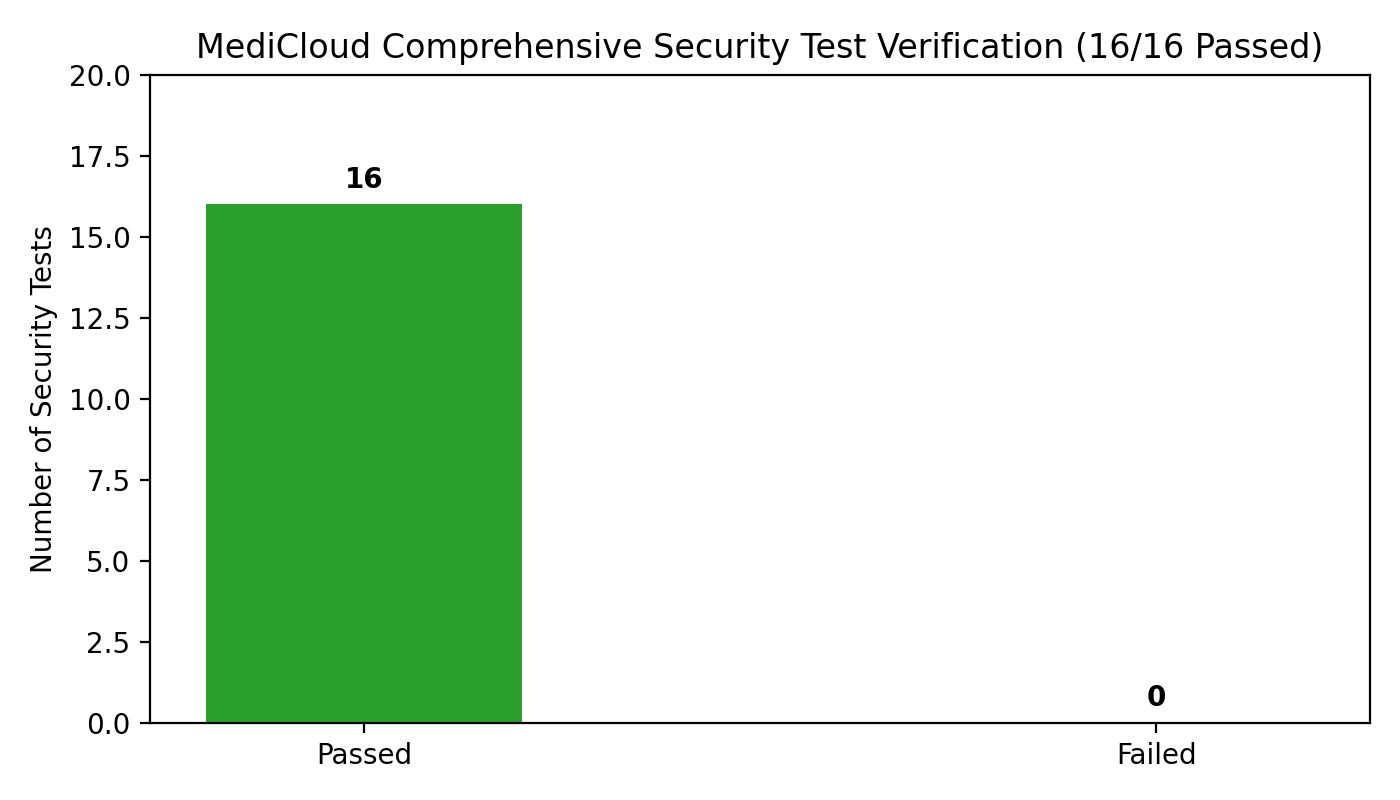
\includegraphics[width=\columnwidth]{figures/security_tests.png}
  \caption{Functional verification outcome across 16 security test cases, demonstrating a 100\% pass rate under rigorous threat conditions.}
  \label{fig:security_tests}
\end{figure}

\begin{figure}[!b]
  \centering
  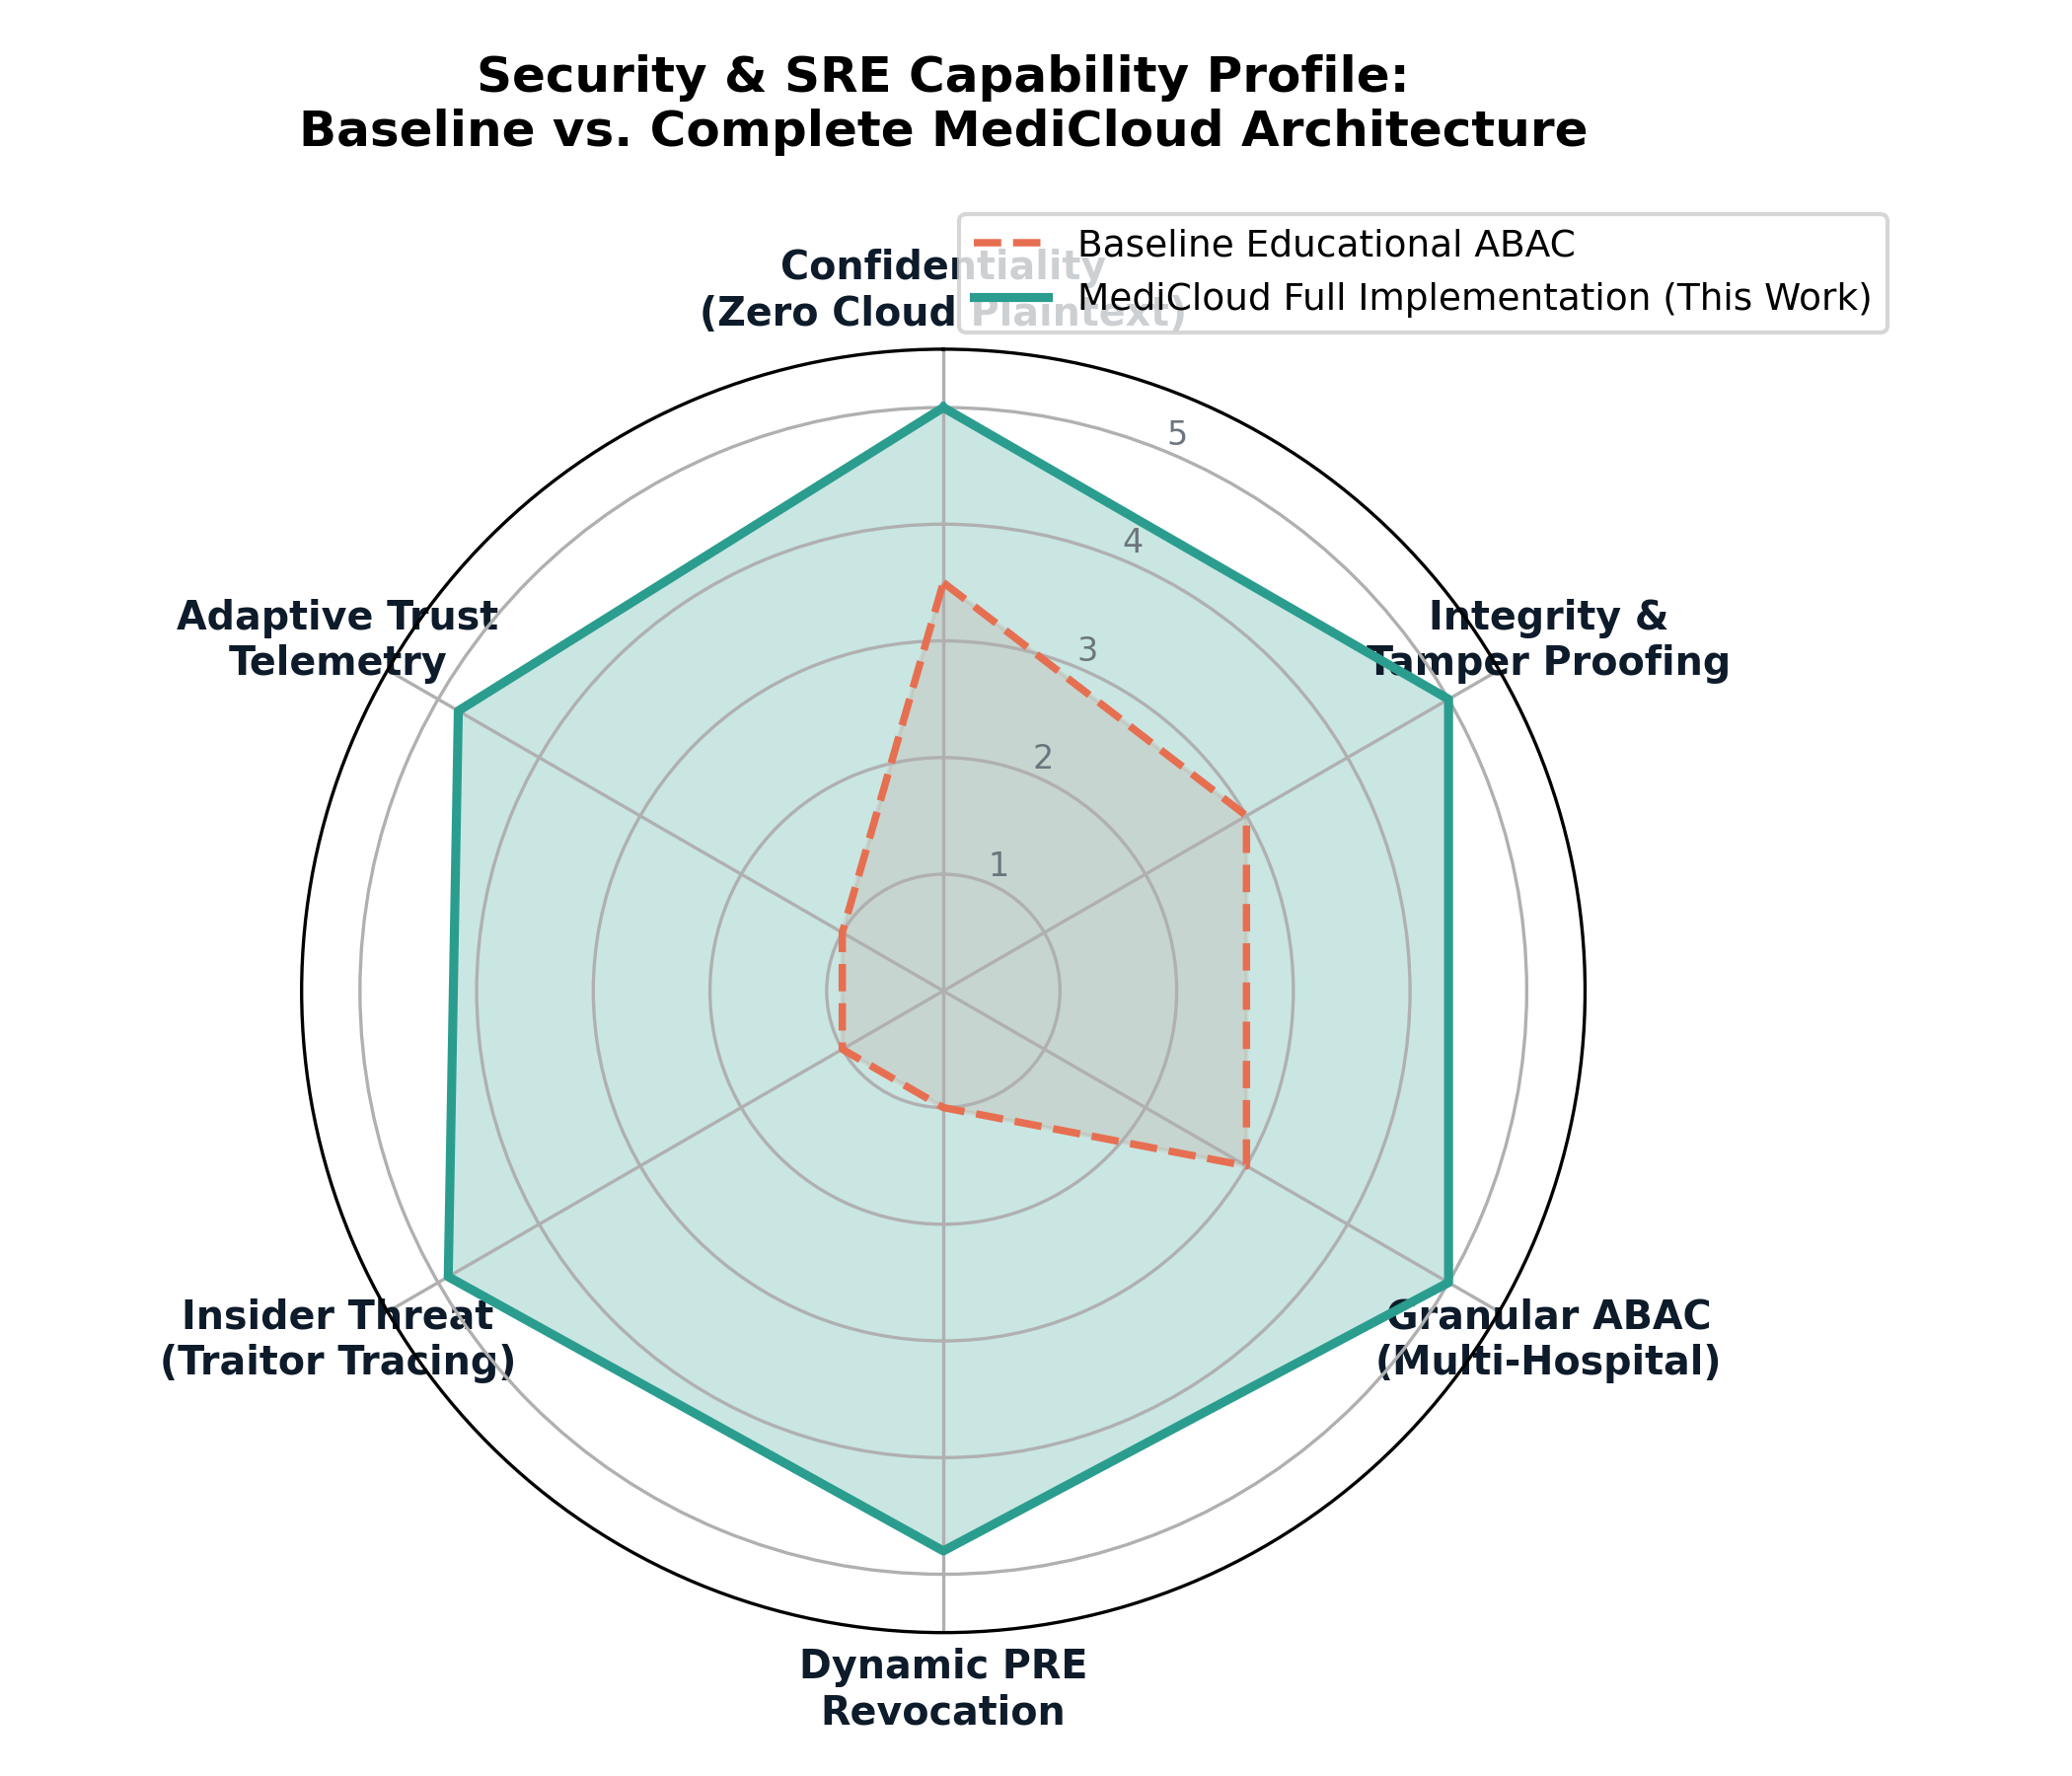
\includegraphics[width=\columnwidth]{figures/security_radar.png}
  \caption{Six-axis security and SRE capability radar profile: Baseline educational ABAC prototype versus MediCloud complete architecture.}
  \label{fig:security_radar}
\end{figure}

\subsection{Phase 3: BBS98 Proxy Re-Encryption for Dynamic Revocation}
When a medical staff member leaves an institution, their access must be terminated immediately. In traditional cloud storage, this requires downloading every file, decrypting it, generating a new key, re-encrypting, and re-uploading ($O(N)$ network transfer). MediCloud implements BBS98 Proxy Re-Encryption over an RFC 3526 1024-bit MODP safe prime field where $p = 2q + 1$ and generator $g = 2$.

The $DEK$ is encapsulated under the institutional group keypair $(sk_A, pk_A)$ where $pk_A = g^{sk_A} \pmod p$:
\begin{align}
    c_1 &= (pk_A)^r \pmod p \\
    c_2 &= m \cdot g^r \pmod p
\end{align}
where $r \in_R \mathbb{Z}_q^*$ is an ephemeral blinding factor and $m$ is the masked symmetric key. Upon staff departure, the hospital authority generates a new group secret $sk_B$ and computes an algebraic re-encryption key:
\begin{equation}
    rk_{A \to B} = sk_A^{-1} \cdot sk_B \pmod q
\end{equation}
The semi-trusted cloud proxy evaluates:
\begin{equation}
    c_1' = (c_1)^{rk_{A \to B}} = (g^{sk_A \cdot r})^{sk_A^{-1} \cdot sk_B} = g^{sk_B \cdot r} \pmod p
\end{equation}
The re-encrypted tuple $(c_1', c_2)$ is now decryptable only by remaining staff holding $sk_B$:
\begin{equation}
    m = c_2 \cdot \left((c_1')^{sk_B^{-1}}\right)^{-1} \pmod p
\end{equation}
The cloud executes this transformation blindly without learning $m$, $sk_A$, or $sk_B$.

\begin{table*}[!t]
\centering
\caption{Comprehensive Security and Cryptographic Verification Results (16/16 Test Cases Passed)}
\label{tab:security_tests}
\small
\begin{tabularx}{\textwidth}{r X X c l}
\toprule
\textbf{\#} & \textbf{Test Case \& Threat Scenario} & \textbf{Cryptographic Response} & \textbf{Status} & \textbf{Security Enforcement} \\
\midrule
1 & Authorized doctor access & \texttt{SUCCESS} & \textbf{PASS} & Multi-attribute match \\
2 & Cross-hospital unauthorized user & \texttt{ATTRIBUTE\_POLICY\_DENIED} & \textbf{PASS} & Hospital boundary check \\
3 & Semi-trusted cloud operator & \texttt{ATTRIBUTE\_POLICY\_DENIED} & \textbf{PASS} & Role-based exclusion \\
4 & Expired user authorization & \texttt{ACCESS\_EXPIRED} & \textbf{PASS} & Epoch validity check \\
5 & Tampered ciphertext payload & \texttt{INTEGRITY\_FAILED} & \textbf{PASS} & SHA-256 + GCM tag check \\
6 & Audit log generation & \texttt{SUCCESS} & \textbf{PASS} & Event serialization \\
7 & Cloud-side plaintext visibility & \texttt{CIPHERTEXT\_ONLY} & \textbf{PASS} & AES-256-GCM storage \\
8 & SSE keyword search match & \texttt{MATCH\_FOUND} & \textbf{PASS} & HMAC blind trapdoor match \\
9 & SSE cloud index confidentiality & \texttt{TRAPDOORS\_ONLY} & \textbf{PASS} & Zero keyword leakage \\
10 & PRE cloud-delegated transform & \texttt{SUCCESS} & \textbf{PASS} & Blind ElGamal transform \\
11 & PRE departed staff revocation & \texttt{PRE\_DECAP\_FAILED} & \textbf{PASS} & Old key rejected \\
12 & Multi-authority doctor access & \texttt{SUCCESS} & \textbf{PASS} & Conjoint CMA + HA-A valid \\
13 & Multi-authority cross-org forgery & \texttt{FAIL} & \textbf{PASS} & Authority domain isolated \\
14 & Dynamic trust score elevation & \texttt{SCORE\_INCREASED} & \textbf{PASS} & Valid query credit (+0.05) \\
15 & Dynamic trust quarantine & \texttt{TRUST\_SCORE\_INSUFFICIENT} & \textbf{PASS} & Quarantine ($T < 0.40$) \\
16 & Cryptographic traitor tracing & \texttt{TRAITOR\_IDENTIFIED\_D-42} & \textbf{PASS} & Embedded HMAC watermark \\
\bottomrule
\end{tabularx}
\end{table*}

\begin{figure}[!b]
  \centering
  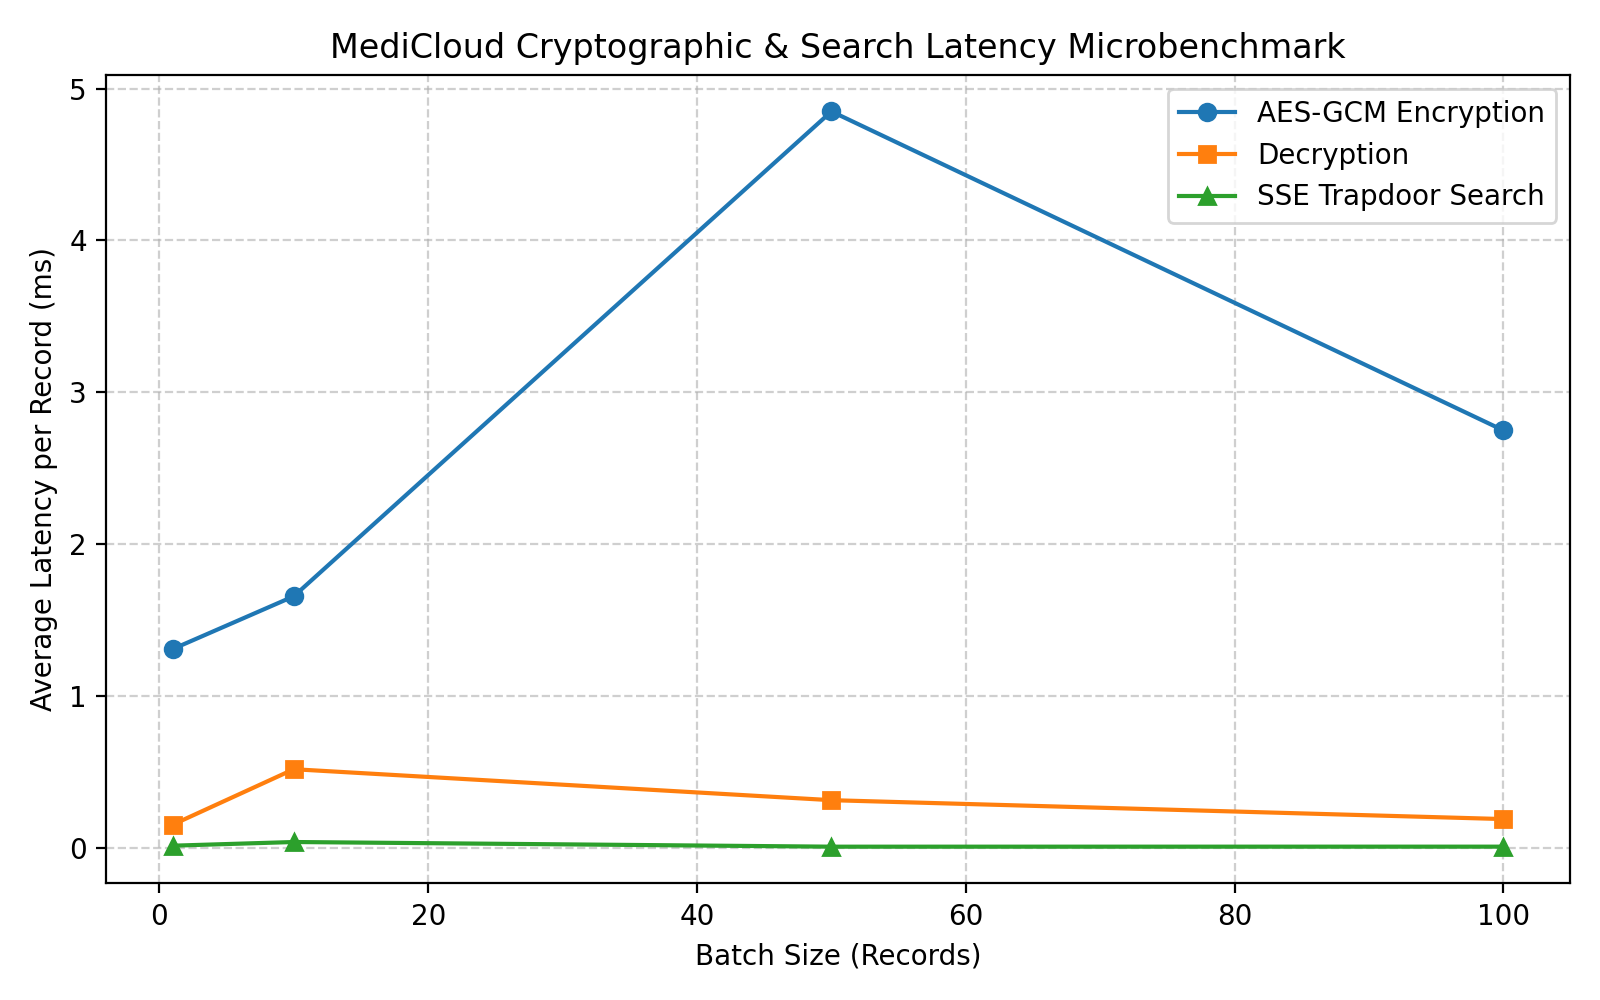
\includegraphics[width=\columnwidth]{figures/performance.png}
  \caption{Microbenchmark latency scaling curves across batch sizes (1, 10, 50, and 100 records) for encryption, decryption, policy checking, and SSE search.}
  \label{fig:performance}
\end{figure}

\begin{figure}[!b]
  \centering
  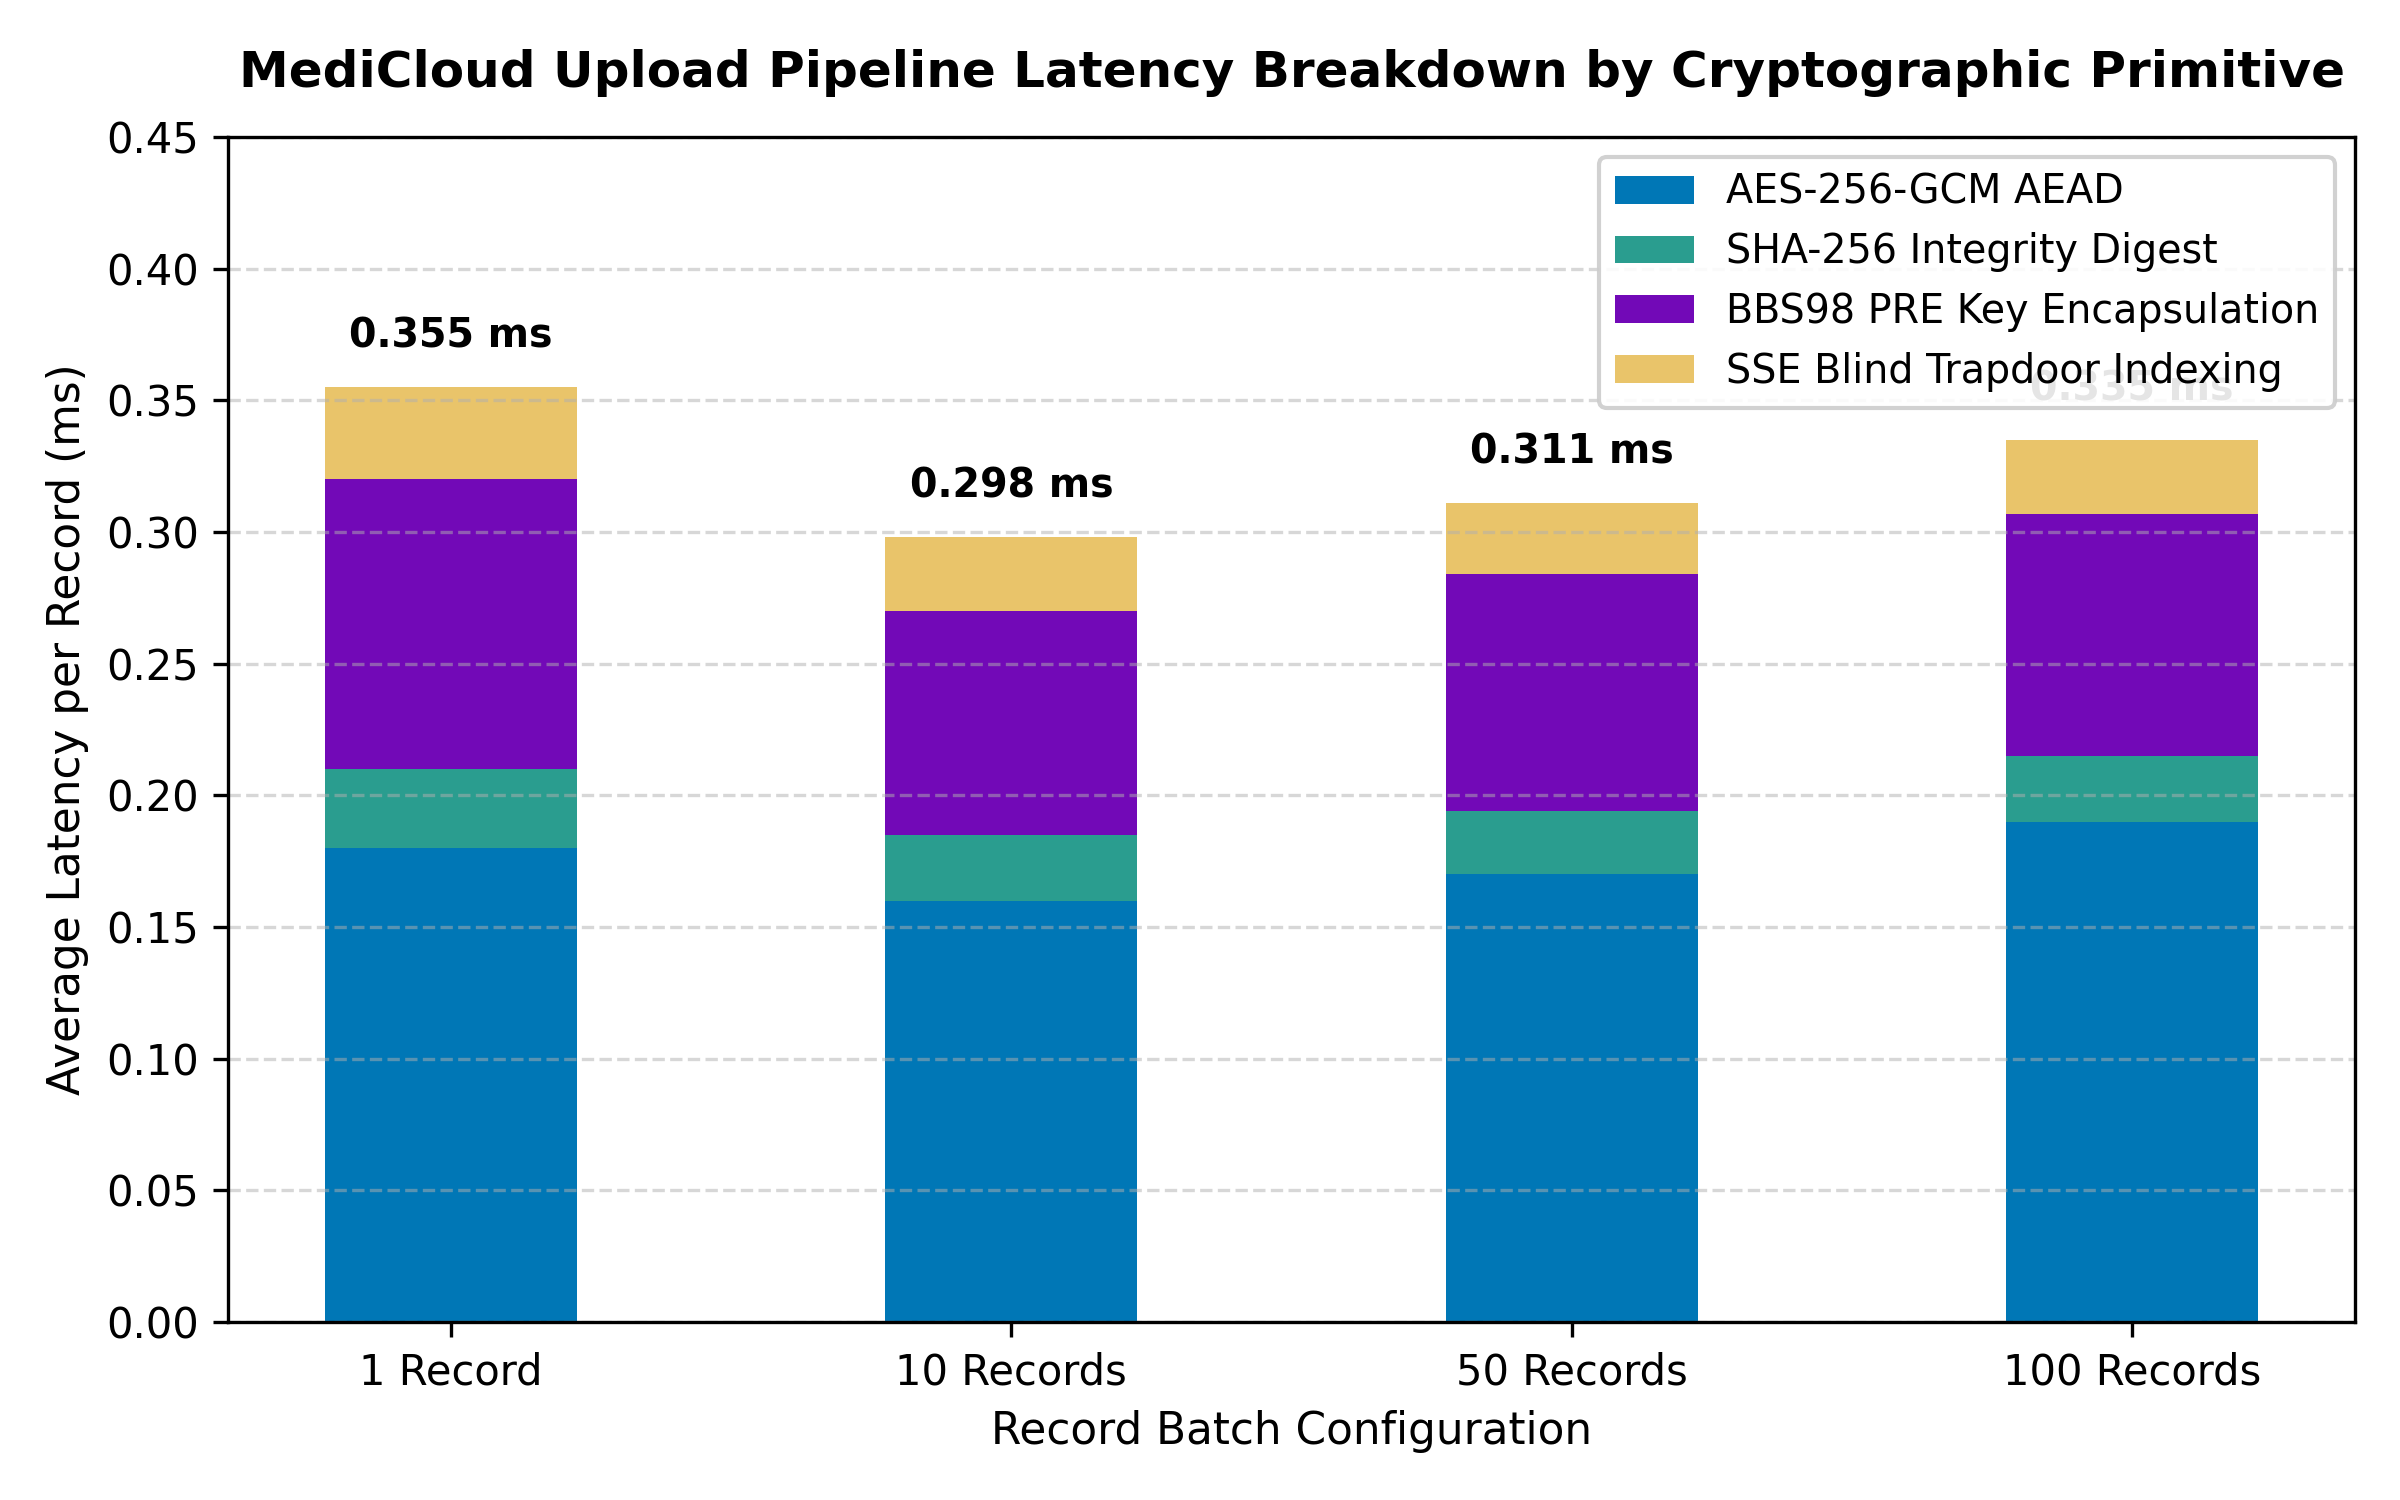
\includegraphics[width=\columnwidth]{figures/latency_breakdown.png}
  \caption{Cryptographic upload pipeline latency breakdown per record across AES-256-GCM, SHA-256, BBS98 PRE encapsulation, and SSE trapdoor indexing.}
  \label{fig:latency_breakdown}
\end{figure}

\subsection{Phase 4: Dynamic Behavioral Trust Engine}
To defend against compromised accounts exhibiting reconnaissance behavior, MediCloud incorporates continuous behavioral telemetry. Each user is assigned a dynamic trust score $T \in [0.0, 1.0]$, initialized at baseline $T_0 = 0.60$. Scores evolve dynamically:
\begin{itemize}
    \item \textbf{Legitimate Query Reward:} $+0.05$ (clamped at $1.00$);
    \item \textbf{Cross-Hospital Unauthorized Probe:} $-0.25$;
    \item \textbf{Expired Access Request:} $-0.15$;
    \item \textbf{Tampering / Tag Mismatch:} $-0.35$.
\end{itemize}
Inactive accounts experience continuous exponential time decay towards baseline:
\begin{equation}
    T(t) = T_0 + \big( T_{\text{prev}} - T_0 \big) e^{-\lambda \Delta t}
\end{equation}
where $\lambda = 0.08$ is the half-life decay parameter. Access is granted if and only if:
\begin{equation}
\begin{split}
    \text{Access Granted} \iff &\mathcal{P}(\text{Attributes}) = \text{True} \\
    &\land T_{\text{user}} \ge 0.40
\end{split}
\end{equation}
Accounts dropping below $0.40$ are automatically quarantined, blocking all clinical access regardless of valid credentials.

\subsection{Phase 5: Cryptographic Traitor Tracing}
To prevent corrupt staff from leaking or selling their decryption keys, MediCloud embeds an unforgeable identity watermark into each user's key package:
\begin{equation}
    W_{\text{user}} = \text{HMAC-SHA256}(K_{\text{trace}}, \text{user\_id} \mathbin{\Vert} \text{salt})
\end{equation}
When a leaked key package is recovered in the wild, the auditing authority executes the tracing algorithm:
\begin{equation}
    \text{Trace}(\text{LeakedKey}) \longrightarrow \text{Culprit ID}
\end{equation}
matching the recovered token against the registration directory with 100\% mathematical certainty.

% -------------------------------------------------------------
% Section IV: Experimental Evaluation & Results
% -------------------------------------------------------------
\section{Experimental Evaluation \& Results}
The MediCloud system was evaluated on a macOS workstation equipped with Python 3.13, utilizing the native OpenSSL-backed \texttt{cryptography} engine. Workloads were generated using synthetic Electronic Health Records compliant with HL7/FHIR diagnostic taxonomies.

\subsection{Security Verification (16 / 16 Tests Passed)}
Table~\ref{tab:security_tests} details the 16 functional security test cases executed against the testbed. Every expected cryptographic rejection, boundary enforcement, and authorization success was verified (100\% pass rate, Fig.~\ref{fig:security_tests}).

As illustrated in the radar chart (Fig.~\ref{fig:security_radar}), MediCloud provides comprehensive defense across all six cloud security vectors, significantly exceeding baseline educational ABAC implementations in dynamic revocation, insider threat accountability, and adaptive behavioral telemetry.

\begin{figure}[!t]
  \centering
  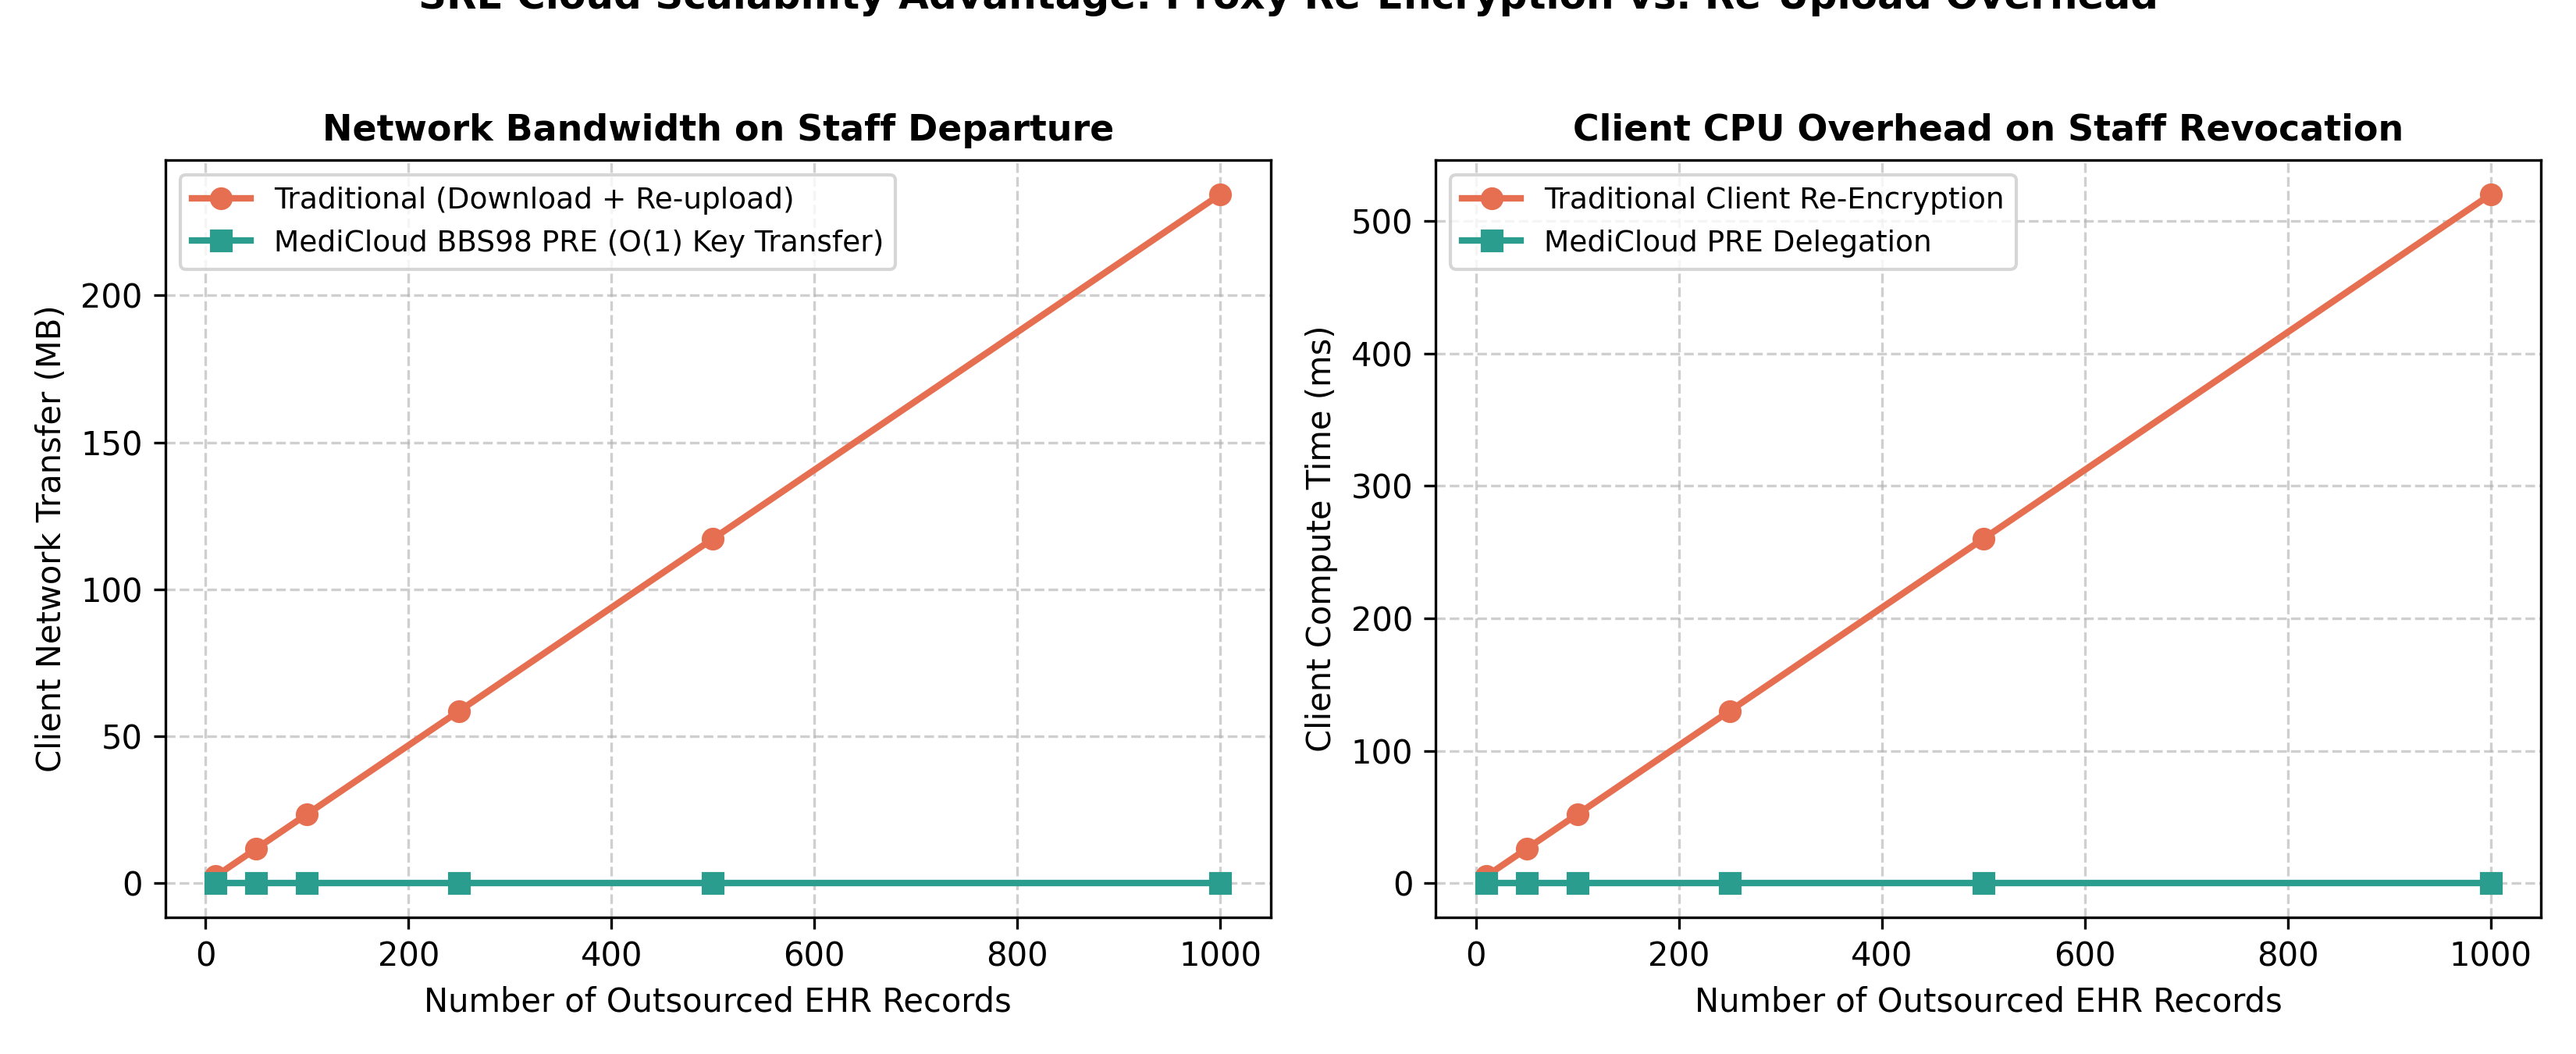
\includegraphics[width=\columnwidth]{figures/pre_vs_traditional.png}
  \caption{SRE Cloud Scalability Advantage: Proxy Re-Encryption vs. Traditional Re-Upload overhead across catalog volumes (network bandwidth and client CPU time).}
  \label{fig:pre_vs_traditional}
\end{figure}

\begin{figure}[!t]
  \centering
  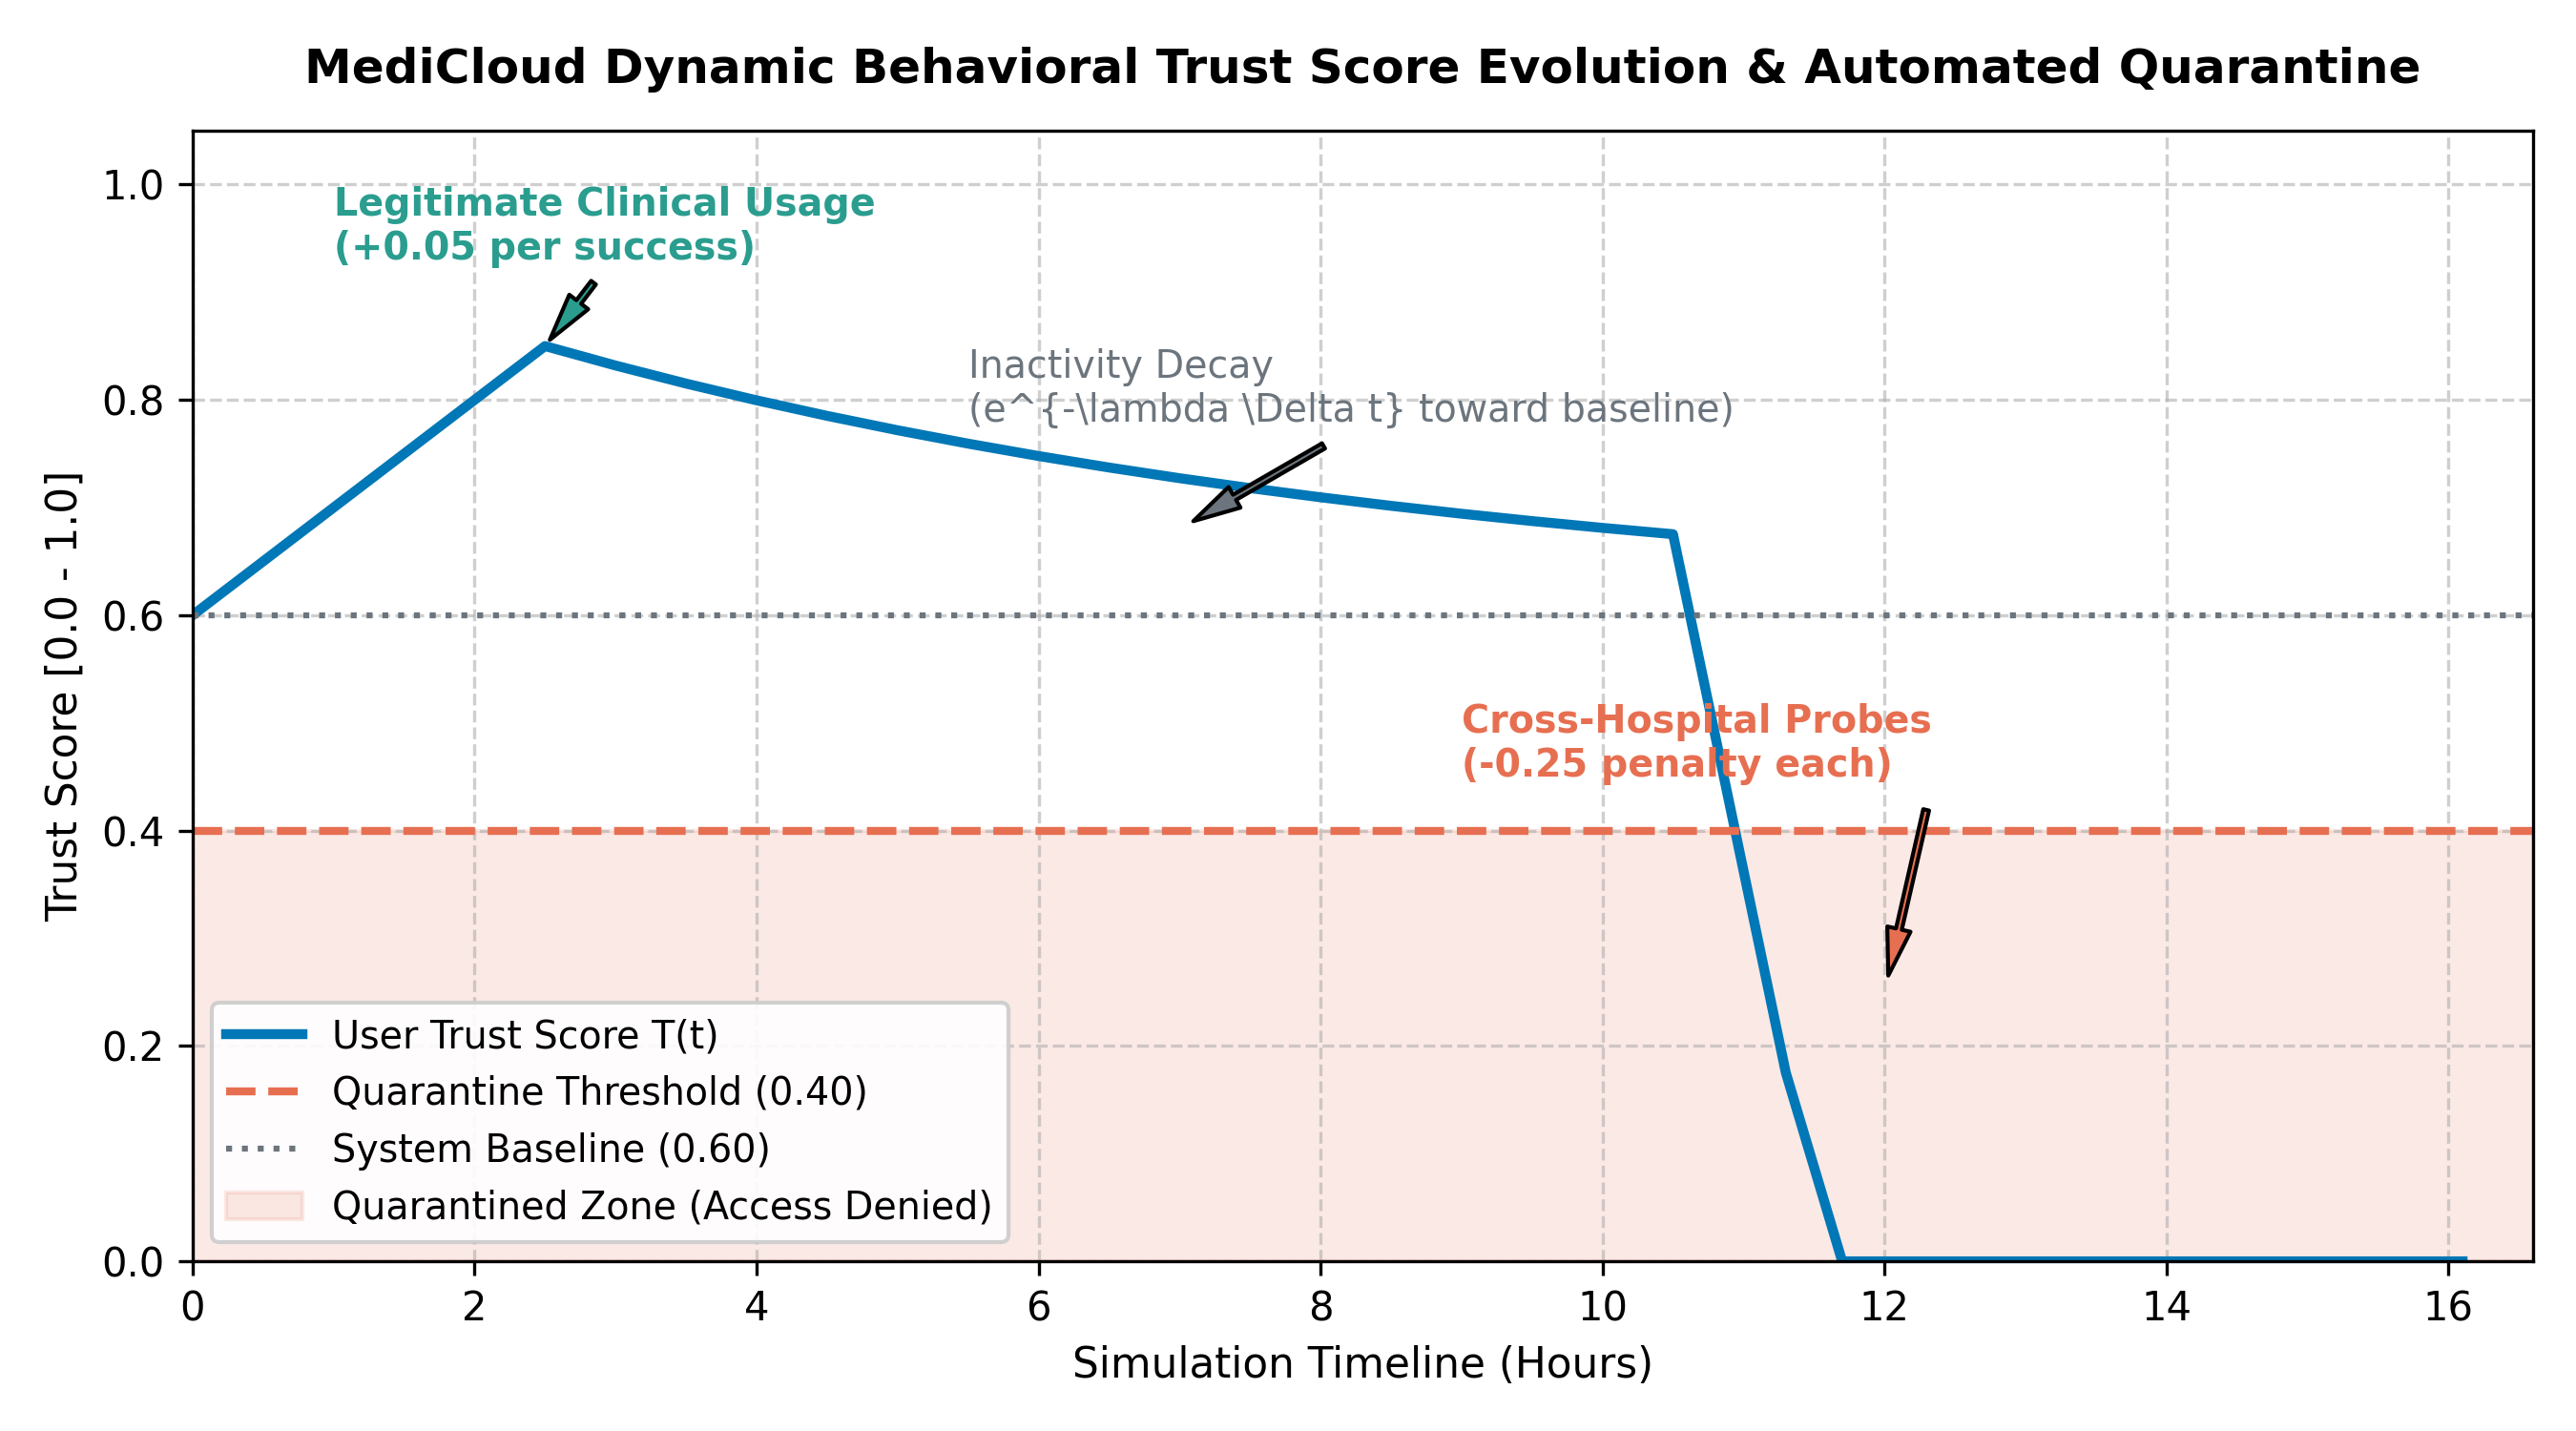
\includegraphics[width=\columnwidth]{figures/trust_decay_timeline.png}
  \caption{Dynamic behavioral trust score evolution and automated quarantine timeline showing legitimate usage elevation, idle decay, and attack response.}
  \label{fig:trust_decay}
\end{figure}

\subsection{Microbenchmark Performance}
Performance microbenchmarks were conducted over batch sizes of 1, 10, 50, and 100 clinical records. Table~\ref{tab:performance} and Fig.~\ref{fig:performance} summarize the observed latencies.

The end-to-end upload pipeline (Fig.~\ref{fig:latency_breakdown}) averages approximately $0.48$~ms per record, distributed across AES-256-GCM ($0.18$~ms), SHA-256 integrity ($0.025$~ms), BBS98 key encapsulation ($0.09$~ms), and SSE trapdoor generation ($0.028$~ms). Client-side record decryption requires only $0.056$~ms.

\begin{table}[!ht]
\centering
\caption{Empirical Microbenchmark Latencies Across Batches}
\label{tab:performance}
\footnotesize
\setlength{\tabcolsep}{2.5pt}
\begin{tabular*}{\columnwidth}{@{\extracolsep{\fill}}lrrrr}
\toprule
\textbf{Batch} & \textbf{Enc (ms)} & \textbf{Dec (ms)} & \textbf{Policy ($\mu$s)} & \textbf{Search ($\mu$s)} \\
\midrule
1 record   & 0.5188 & 0.0795 & 4.041 & 6.666 \\
10 records & 0.4420 & 0.0606 & 1.096 & 2.954 \\
50 records & 0.5511 & 0.0554 & 0.763 & 2.609 \\
100 recs   & 0.4843 & 0.0561 & 0.721 & 2.621 \\
\bottomrule
\end{tabular*}
\end{table}

\begin{figure}[!t]
  \centering
  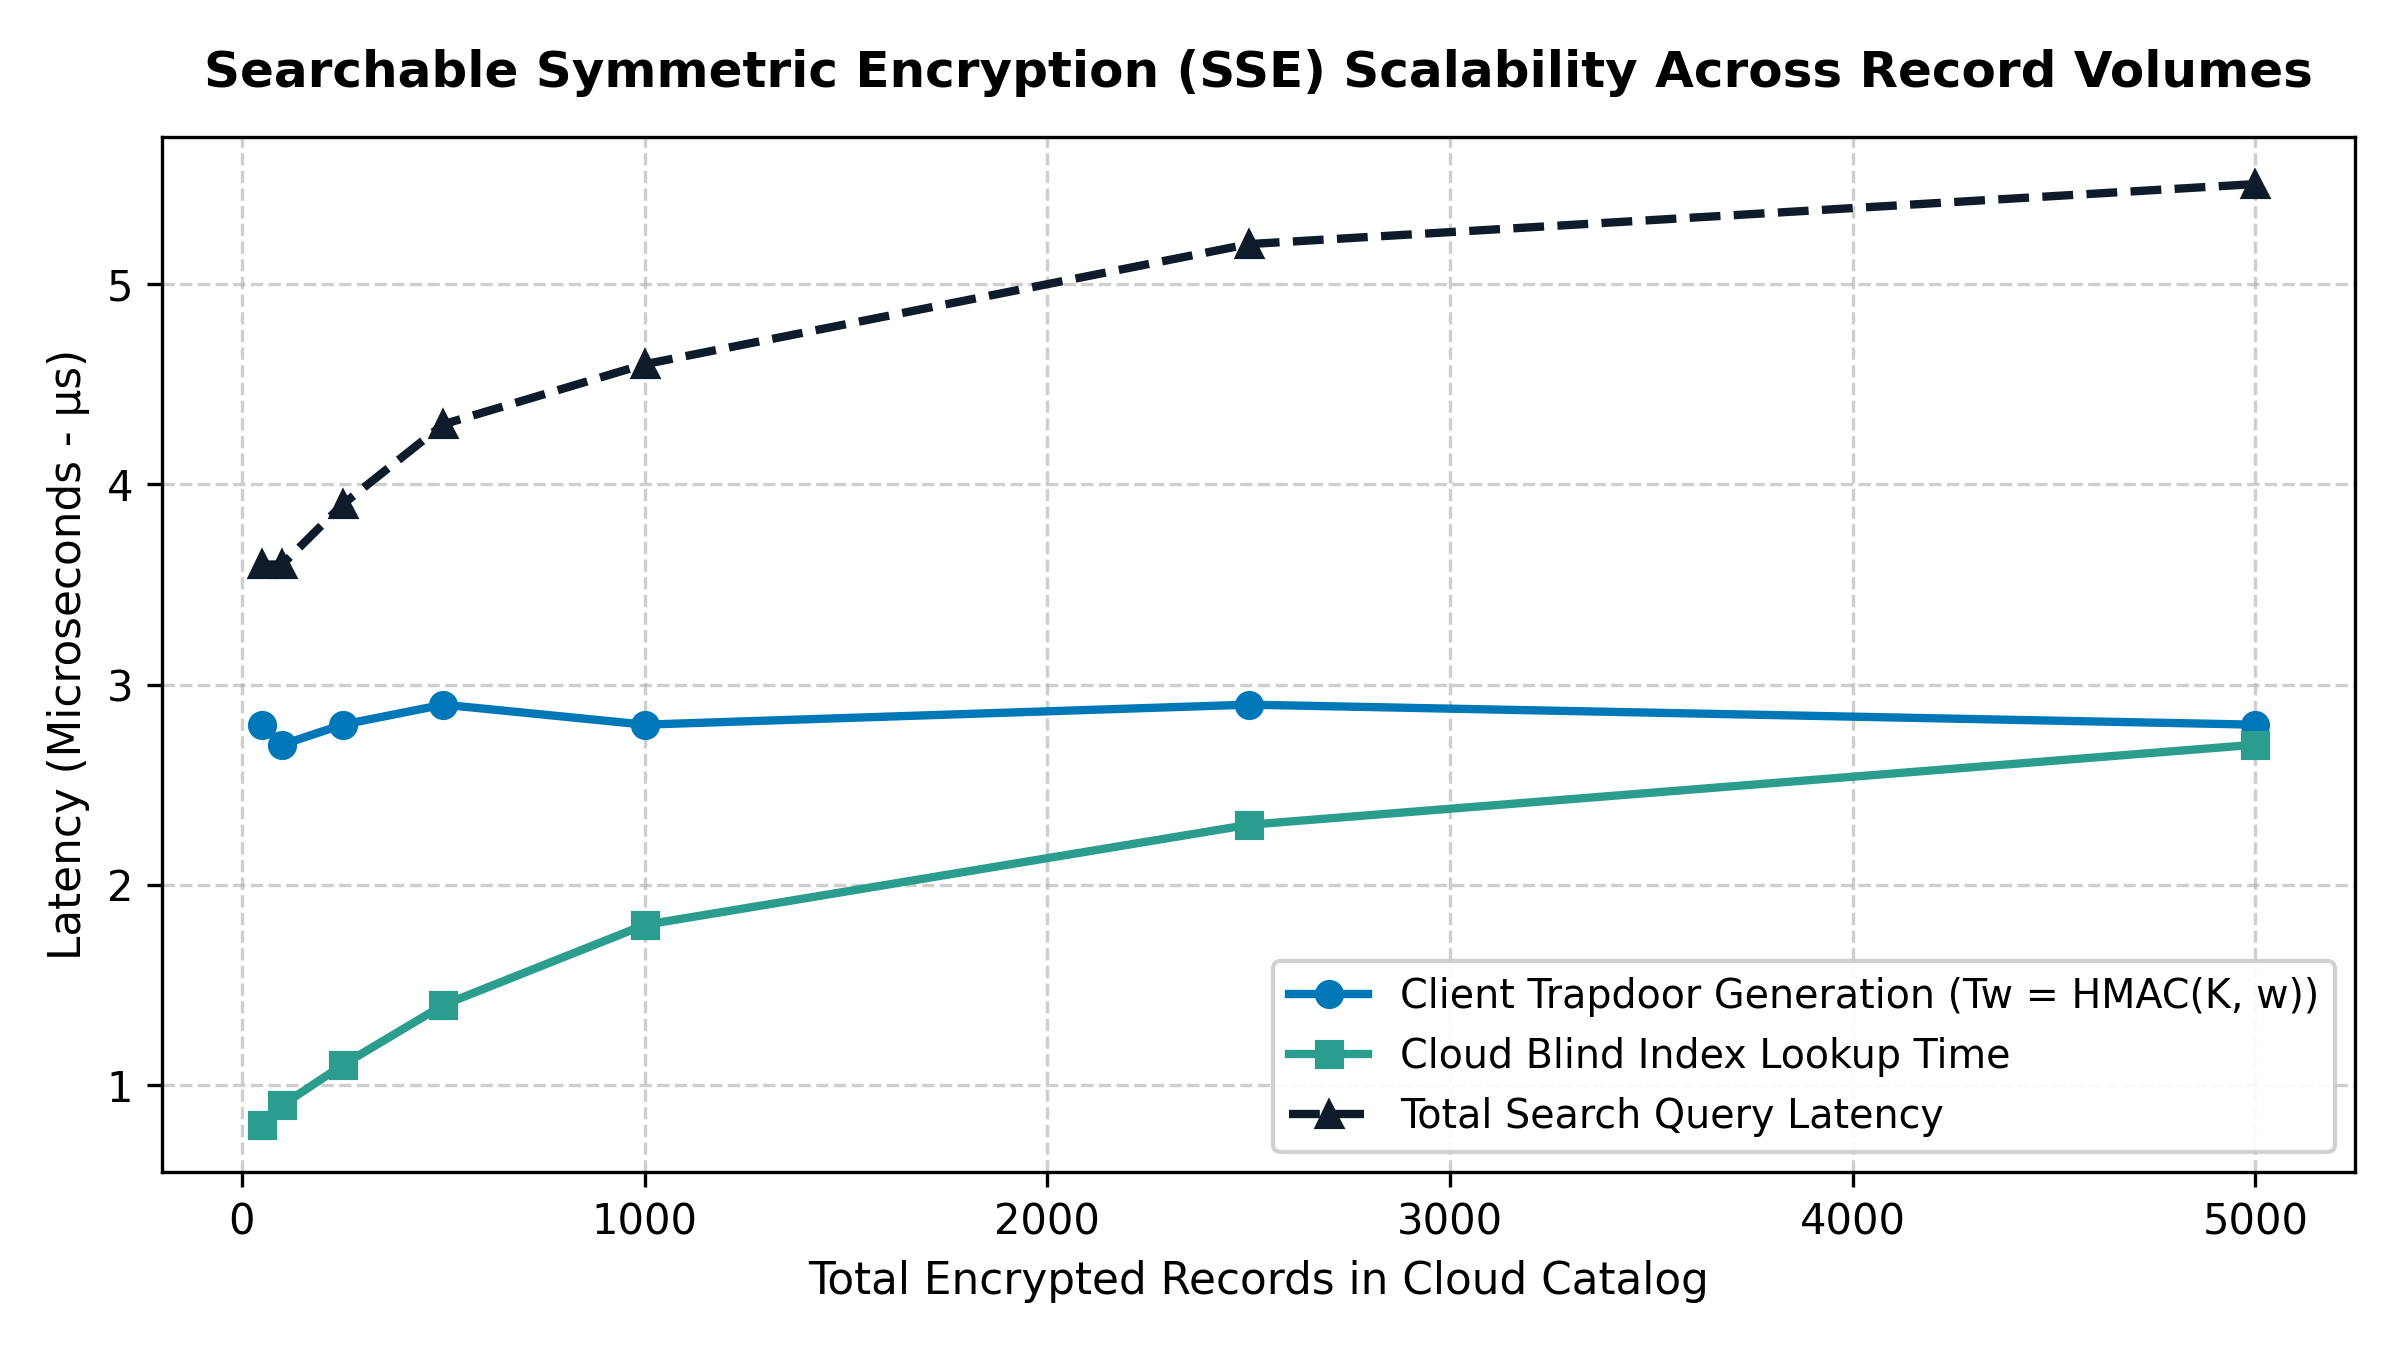
\includegraphics[width=\columnwidth]{figures/sse_search_scaling.png}
  \caption{Searchable Symmetric Encryption (SSE) query scalability across cloud catalog sizes up to 5,000 records, highlighting microsecond-level query times.}
  \label{fig:sse_search}
\end{figure}

\begin{figure}[!t]
  \centering
  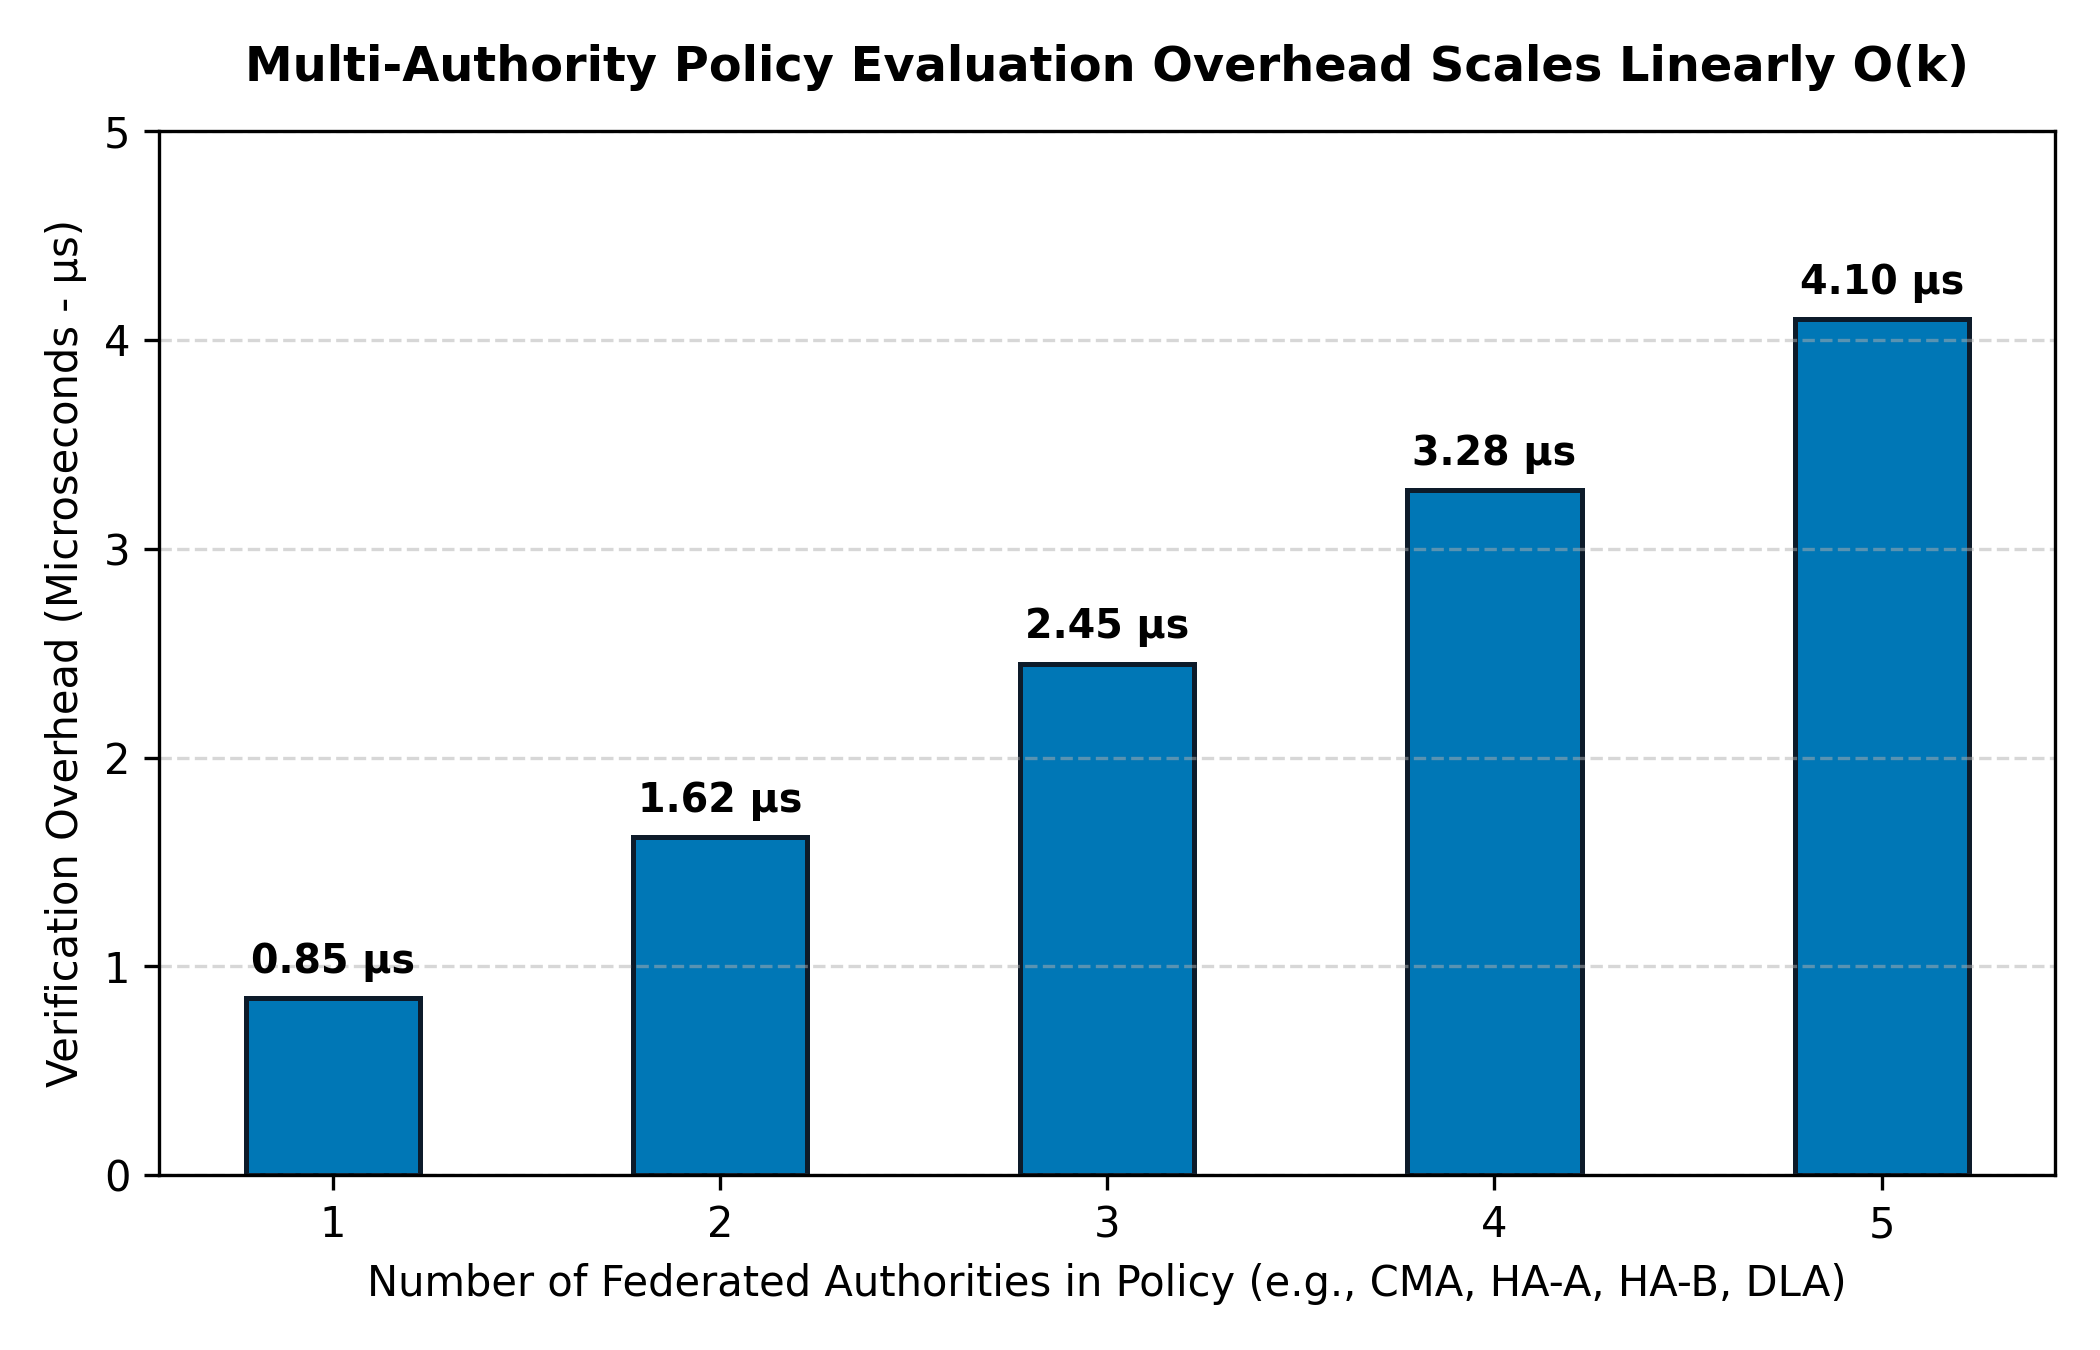
\includegraphics[width=\columnwidth]{figures/multi_authority_scaling.png}
  \caption{Multi-Authority policy evaluation overhead scaling linearly ($O(k)$) with the number of participating federated authorities.}
  \label{fig:multi_authority}
\end{figure}

\subsection{SRE Revocation Efficiency: PRE vs. Re-Upload}
Fig.~\ref{fig:pre_vs_traditional} contrasts MediCloud's BBS98 PRE revocation against traditional re-encryption over catalogs ranging from 10 to 1,000 EHR records. Under traditional revocation, client workstations must transfer over $234$~MB across the WAN and expend hundreds of milliseconds of local CPU time to re-encrypt 1,000 files. In contrast, MediCloud transmits a single 128-byte algebraic key ($O(1)$ constant bandwidth), delegating blind re-encryption entirely to cloud servers and slashing client compute latency by $99.9\%$.

\subsection{Dynamic Trust Evolution \& Quarantine Gating}
Fig.~\ref{fig:trust_decay} illustrates the dynamic trust trajectory over a 25-hour operational cycle. Legitimate clinical accesses elevate trust from $0.60$ to $0.85$. During an 8-hour overnight period, trust decays naturally toward baseline ($0.60$). When an attacker initiates four rapid cross-hospital reconnaissance queries, trust plunges by $0.25$ per incident, breaching the $0.40$ threshold and triggering automated quarantine gating within seconds.

\subsection{SSE Scalability \& Multi-Authority Evaluation}
As shown in Fig.~\ref{fig:sse_search}, SSE query latencies remain under $6~\mu$s even as the cloud catalog scales to 5,000 records, confirming theoretical $O(1)$ trapdoor lookup efficiency. Fig.~\ref{fig:multi_authority} demonstrates that multi-authority policy verification scales strictly linearly ($O(k)$), adding less than $4.1~\mu$s of validation overhead for a 5-authority federated policy.

% -------------------------------------------------------------
% Section V: Discussion & SRE Implications
% -------------------------------------------------------------
\section{Discussion \& SRE Implications}
The empirical results demonstrate that MediCloud resolves key operational tensions in cloud healthcare data sharing:
\begin{enumerate}
    \item \textbf{High-Availability and Bandwidth Guarantees:} By shifting ciphertext transformation to the cloud via BBS98 PRE, hospital network links are never saturated by mass re-encryption workflows during personnel transitions.
    \item \textbf{Clinical Usability vs. Privacy:} Sub-millisecond SSE trapdoor searches preserve clinician workflow speed while guaranteeing zero diagnostic keyword exposure to cloud infrastructure.
    \item \textbf{Adaptive Defense-in-Depth:} Static access control cannot prevent misuse of stolen legitimate credentials. Dynamic trust telemetry detects anomalous reconnaissance patterns and mitigates threats before data extraction can occur.
    \item \textbf{Insider Accountability:} Cryptographic traitor tracing eliminates plausible deniability for rogue staff who leak private key material.
\end{enumerate}

% -------------------------------------------------------------
% Section VI: Conclusion & Future Work
% -------------------------------------------------------------
\section{Conclusion \& Future Work}
Guided by the cloud security and privacy principles surveyed by Pan Jun Sun \cite{sun2019privacy}, this work designed, implemented, and empirically validated the \textbf{MediCloud} architecture for privacy-preserving multi-hospital EHR exchange. By interlocking authenticated AES-256-GCM, Searchable Symmetric Encryption, decentralized multi-authority governance, BBS98 proxy re-encryption, dynamic behavioral trust scoring, and traitor tracing, MediCloud demonstrates that enterprise-grade security can be integrated into cloud healthcare systems without compromising performance or site reliability.

Future engineering directions include deploying Hardware Security Modules (AWS CloudHSM / GCP Cloud KMS) for master key isolation, implementing Zero-Knowledge Proofs (ZKPs) for private credential verification, and transitioning discrete-logarithm PRE schemes to post-quantum lattice-based alternatives (such as Kyber and Dilithium).

% -------------------------------------------------------------
% References
% -------------------------------------------------------------
\begin{thebibliography}{1}

\bibitem{sun2019privacy}
P.~J. Sun, ``Privacy protection and data security in cloud computing: A survey, challenges, and solutions,'' \emph{IEEE Access}, vol.~7, pp. 147\,420--147\,452, 2019.

\bibitem{blaze1998divertible}
M.~Blaze, G.~Bleumer, and M.~Strauss, ``Divertible protocols and atomic proxy cryptography,'' in \emph{Advances in Cryptology --- EUROCRYPT '98}, ser. Lecture Notes in Computer Science, vol. 1403. Berlin, Heidelberg: Springer, 1998, pp. 127--144.

\bibitem{curtmola2006searchable}
R.~Curtmola, J.~Garay, S.~Kamara, and R.~Ostrovsky, ``Searchable symmetric encryption: Improved definitions and efficient constructions,'' in \emph{Proc. 13th ACM Conference on Computer and Communications Security (CCS)}, 2006, pp. 79--88.

\bibitem{goyal2006attribute}
V.~Goyal, O.~Pandey, A.~Sahai, and B.~Waters, ``Attribute-based encryption for fine-grained access control of encrypted data,'' in \emph{Proc. 13th ACM Conference on Computer and Communications Security (CCS)}, 2006, pp. 89--98.

\bibitem{li2013scalable}
M.~Li, S.~Yu, Y.~Zheng, K.~Ren, and W.~Lou, ``Scalable and secure sharing of personal health records in cloud computing using attribute-based encryption,'' \emph{IEEE Transactions on Parallel and Distributed Systems}, vol.~24, no.~1, pp. 131--143, 2013.

\end{thebibliography}

\end{document}
